%% Time-stamp: <2018-10-18 20:24:12 (marc)>
\documentclass[xcolor=x11names,compress, mathserif]{beamer}

\newcommand{\hackspace}{\hspace{4.2mm}}
\newcommand{\showstudent}[1]{}
\newcommand\hmmax{0}
\newcommand\bmmax{0}





% talk/author information
\newcommand{\authorname}{Yingzhen Li}
\newcommand{\authoremail}{yingzhen.li@imperial.ac.uk}
\newcommand{\authortwitter}{liyzhen2}
\newcommand{\authoraffiliation}{
  Department of Computing\\Imperial
  College London}
\newcommand{\slidesettitle}{\imperialBlue{Principal Component Analysis}}
\newcommand{\footertitle}{Principal Component Analysis (PCA)}
\newcommand{\location}{Imperial College London}
\newcommand{\talkDate}{Nov 21, 2022}



\date{\imperialGray{\talkDate}}




% load defaults
%\usepackage{../MarkMathCmds}
\selectcolormodel{rgb}
\usepackage{ifxetex,ifluatex}
\newif\ifxetexorluatex
\ifxetex
  \xetexorluatextrue
\else
  \ifluatex
    \xetexorluatextrue
  \else
    \xetexorluatexfalse
  \fi
\fi

\usepackage{textpos}
%\usepackage{arabtex}
\usepackage{tikz}
\usetikzlibrary{decorations.markings}
\usetikzlibrary{arrows}
\usetikzlibrary{shapes}
\usetikzlibrary{plotmarks}
\usetikzlibrary{mindmap,trees,backgrounds}

\tikzstyle{every picture}+=[remember picture]

%\usepackage{movie15}
% \usepackage{pdfpages}
%\usepackage{xmpmulti}

\usepackage{anyfontsize}
\usepackage{wrapfig}
\usepackage{animate}
\usepackage{multirow}
\usepackage{multimedia}
\usepackage{xmpmulti}
%\usepackage[latin9]{inputenc}
\usepackage[english]{babel}
\usepackage{scalefnt}
\usepackage{verbatim}
\usepackage{url}
% \usepackage{pgf,pgfarrows,pgfnodes}
\usepackage{textpos}
\usepackage[tight,ugly]{units}
\usepackage{url}
\usepackage{bbm}
\usepackage[english]{babel}
\usepackage{fancyhdr}
\usepackage{bm} % correct bold symbols, like \bm
\usepackage{amsmath}
\usepackage{amsfonts}
\usepackage{amssymb}
\usepackage{mathrsfs}
\usepackage{mathtools}
\usepackage{color}
\usepackage{cancel}
\usepackage{algorithm}
\usepackage{algpseudocode}
\usepackage{mathrsfs}
\usepackage{listings}
\usepackage{graphicx} % for pdf, bitmapped graphics files
\usepackage{mathtools}
\usepackage{units}
\usepackage{subfig}
\usepackage{enumerate}
\usepackage[comma,authoryear]{natbib}
\usepackage{dsfont}


\ifxetexorluatex
\usepackage{fontspec}
\setmainfont[Scale=0.8]{OpenDyslexic-Regular}
\else
\usefonttheme{professionalfonts}
\fi

\renewcommand{\vec}[1]{{\boldsymbol{{#1}}}} % vector
\newcommand{\mat}[1]{{\boldsymbol{{#1}}}} % matrix
% \newcommand{\KL}[2]{\mathrm{KL}(#1\|#2)} % KL divergence
\newcommand{\R}[0]{\mathds{R}} % real numbers
\newcommand{\Z}[0]{\mathds{Z}} % integers
\newcommand{\tr}[0]{\text{tr}} % trace
% \newcommand{\inv}{^{-1}}
% \DeclareMathOperator*{\diag}{diag}
\newcommand{\E}{\mathds{E}} % expectation
\newcommand{\var}{\mathds{V}}
\newcommand{\gauss}[2]{\mathcal{N}\big(#1,\,#2\big)}
\newcommand{\gaussx}[3]{\mathcal{N}\big(#1\,|\,#2,\,#3\big)}
\newcommand{\gaussBig}[2]{\mathcal{N}\left(#1,\,#2\right)}
\newcommand{\gaussxBig}[3]{\mathcal{N}\left(#1\,\left|\,#2,\,#3\right.\right)}
\newcommand{\Ber}[0]{\mathrm{Ber}} % Bernoulli distribution
\DeclareMathOperator{\cov}{Cov}
\ifxetexorluatex
\renewcommand{\T}[0]{^\top}
\renewcommand{\d}[0]{\text{d}} % derivative
\else
\newcommand{\T}[0]{^\top}
\renewcommand{\d}[0]{\text{d}} % derivative
\fi
% calculus
\newcommand{\pdiff}[1]{\frac{\partial}{\partial #1}}
\newcommand{\pdiffF}[2]{\frac{\partial #1}{\partial #2}}
\newcommand{\diffF}[2]{\frac{{\d}#1}{{\d}#2}}
\newcommand{\diffFII}[2]{\frac{{\d}^2 #1}{{\d}#2^2}}
\newcommand{\diff}[1]{\frac{{\d}}{{\d}#1}}
\newcommand{\diffII}[1]{\frac{{\d}^2}{{\d}#1^2}}
\newcommand{\class}[0]{\mathcal{C}}

\newcommand{\idx}[1]{{(#1)}}
% \newcommand{\norm}[1]{\left\|#1\right\|}
\newcommand{\proj}[1]{\tilde{#1}}
\newcommand{\pcacoord}{z}
\newcommand{\pcacoordnew}{\zeta}
\newcommand{\latent}{z}
% \newcommand{\given}{\,|\,}
\newcommand{\genset}[1]{\mathrm{span}[#1]} % generating set
\newcommand{\set}[1]{\mathcal{#1}} % set
\newcommand{\fixgmfont}[1]{\scalebox{0.8}{#1}}



\usepackage{pifont}% http://ctan.org/pkg/pifont
\newcommand{\cmark}{{\color{green!40!black}\ding{51}}}%
\newcommand{\xmark}{{\color{red}\ding{55}}}%
\newcommand{\green}[1]{{\bf{\textcolor{green}{#1}}}}
\newcommand{\red}[1]{{\bf{\textcolor{red}{#1}}}}

\newcommand<>\red[1]{{\color#2[rgb]{1,0,0}#1}}
\newcommand<>\blue[1]{{\color#2[rgb]{0,0,1}#1}}
\newcommand<>\yellow[1]{{\color#2{camyellow}#1}}
\newcommand<>\green[1]{{\color#2[rgb]{0,0.6,0.0}#1}}
\newcommand<>\violet[1]{{\color#2[rgb]{0.6,0,0.6}#1}}
\newcommand<>\orange[1]{{\color#2[rgb]{1,0.5,0}#1}}
\newcommand<>\black[1]{{\color#2[rgb]{0,0,0}#1}}
\newcommand<>\steel[1]{{\color#2[rgb]{0,0,0.8}#1}}
\newcommand<>\darkblue[1]{{\color#2[rgb]{0,0,0.6}#1}}
\newcommand<>\lightblue[1]{{\color#2[rgb]{0.4,0.4,0.7}#1}}
\newcommand<>\gray[1]{{\color#2[rgb]{0.4,0.4,0.4}#1}}
\newcommand<>\greenish[1]{{\color#2[rgb]{0.45, 0.66, 0.45}#1}}
\newcommand<>\redish[1]{{\color#2[rgb]{0.7843    0.3706    0.3706}#1}}
\definecolor{redishTIKZ}{rgb}{0.7843, 0.3706, 0.3706}
\definecolor{imperialBlue}{rgb}{0.058, 0.219, 0.418}
\definecolor{aimsbrown}{rgb}{0.539, 0.117, 0.015}
% \definecolor{imperialGray}{rgb}{0.414, 0.488, 0.671 }
\definecolor{imperialGray}{RGB}{109,153, 204}
\definecolor{aimslightbrown}{RGB}{138,88,84}
\newcommand<>\imperialBlue[1]{{\color#2[rgb]{0.058, 0.219, 0.418}#1}}
\newcommand<>\aimsbrown[1]{{\color#2[rgb]{0.539, 0.117, 0.015}#1}}
%\newcommand<>\imperialGray[1]{{\color#2[rgb]{0.414, 0.488, 0.671}#1}}
\newcommand<>\imperialGray[1]{{\color#2[RGB]{109,153, 204}#1}}
\newcommand<>\aimslightbrown[1]{{\color#2[RGB]{138,88,84}#1}}
\newcommand<>\lightgray[1]{{\color#2[rgb]{0.8,0.8,0.8}#1}}
%\newcommand<>\highlightcolor[1]{{\color#2[rgb]{0,0,1}#1}}
\newcommand{\highlight}[1]{{\bf\steel{#1}}}
%\newcommand{\newblock}[0]{}

%\newcommand{\arrow}[0]{\includegraphics[height=5pt]{./figures/arrow}\hspace{3pt}}

\renewcommand{\emph}[1]{\textbf{\steel{{#1}}}}

\renewcommand{\alert}[1]{{\bf\red{{#1}}}}

\newcommand{\arrow}{
\begin{tikzpicture}
\draw [black!40!green, fill=black!40!green] (0,-0.12) -- (0,0.12) --
(0.15,0);
\draw [black!40!green, fill=black!40!green] (0.15,-0.12) -- (0.15,0.12) --
(0.3,0); 
\end{tikzpicture}
}

\geometry{left=0.45cm,top=0cm,right=0.45cm}


\newcommand{\logoimagepath}{./figures/imperial}
\newcommand{\highlightcolor}{blue!80!black}
%\newcommand{\headbarcolor}{imperialBlue}
\newcommand{\headbarcolor}{imperialBlue}
\institute{}

\newcommand{\coursetitle}{}

\newcommand{\slidesetsubtitle}{}
\newcommand{\slidesetnumber}{01}
\usefonttheme{professionalfonts}


\usetikzlibrary{decorations.fractals}
% tikzlibrary.code.tex
%
% Copyright 2010-2011 by Laura Dietz
% Copyright 2012 by Jaakko Luttinen
%
% The MIT License
%
% See LICENSE file for more details.

% Load other libraries
\usetikzlibrary{shapes}
\usetikzlibrary{fit}
\usetikzlibrary{chains}
\usetikzlibrary{arrows}

% Latent node
\tikzstyle{latent} = [circle,fill=white,draw=black,inner sep=1pt,
minimum size=20pt, font=\fontsize{10}{10}\selectfont, node distance=1]
% Observed node
\tikzstyle{obs} = [latent,fill=gray!25]
% Constant node
\tikzstyle{const} = [rectangle, inner sep=0pt, node distance=1]
% Factor node
\tikzstyle{factor} = [rectangle, fill=black,minimum size=5pt, inner
sep=0pt, node distance=0.4]
% Deterministic node
\tikzstyle{det} = [latent, diamond]

% Plate node
\tikzstyle{plate} = [draw, rectangle, rounded corners, fit=#1]
% Invisible wrapper node
\tikzstyle{wrap} = [inner sep=0pt, fit=#1]
% Gate
\tikzstyle{gate} = [draw, rectangle, dashed, fit=#1]

% Caption node
\tikzstyle{caption} = [font=\footnotesize, node distance=0] %
\tikzstyle{plate caption} = [caption, node distance=0, inner sep=0pt,
below left=5pt and 0pt of #1.south east] %
\tikzstyle{factor caption} = [caption] %
\tikzstyle{every label} += [caption] %

%\pgfdeclarelayer{b}
%\pgfdeclarelayer{f}
%\pgfsetlayers{b,main,f}

% \factoredge [options] {inputs} {factors} {outputs}
\newcommand{\factoredge}[4][]{ %
  % Connect all nodes #2 to all nodes #4 via all factors #3.
  \foreach \f in {#3} { %
    \foreach \x in {#2} { %
      \path (\x) edge[-,#1] (\f) ; %
      %\draw[-,#1] (\x) edge[-] (\f) ; %
    } ;
    \foreach \y in {#4} { %
      \path (\f) edge[->, >={triangle 45}, #1] (\y) ; %
      %\draw[->,#1] (\f) -- (\y) ; %
    } ;
  } ;
}

% \edge [options] {inputs} {outputs}
\newcommand{\edge}[3][]{ %
  % Connect all nodes #2 to all nodes #3.
  \foreach \x in {#2} { %
    \foreach \y in {#3} { %
      \path (\x) edge [->, >={triangle 45}, #1] (\y) ;%
      %\draw[->,#1] (\x) -- (\y) ;%
    } ;
  } ;
}

% \factor [options] {name} {caption} {inputs} {outputs}
\newcommand{\factor}[5][]{ %
  % Draw the factor node. Use alias to allow empty names.
  \node[factor, label={[name=#2-caption]#3}, name=#2, #1,
  alias=#2-alias] {} ; %
  % Connect all inputs to outputs via this factor
  \factoredge {#4} {#2-alias} {#5} ; %
}

% \plate [options] {name} {fitlist} {caption}
\newcommand{\plate}[4][]{ %
  \node[wrap=#3] (#2-wrap) {}; %
  \node[plate caption=#2-wrap] (#2-caption) {#4}; %
  \node[plate=(#2-wrap)(#2-caption), #1] (#2) {}; %
}

% \gate [options] {name} {fitlist} {inputs}
\newcommand{\gate}[4][]{ %
  \node[gate=#3, name=#2, #1, alias=#2-alias] {}; %
  \foreach \x in {#4} { %
    \draw [-*,thick] (\x) -- (#2-alias); %
  } ;%
}

% \vgate {name} {fitlist-left} {caption-left} {fitlist-right}
% {caption-right} {inputs}
\newcommand{\vgate}[6]{ %
  % Wrap the left and right parts
  \node[wrap=#2] (#1-left) {}; %
  \node[wrap=#4] (#1-right) {}; %
  % Draw the gate
  \node[gate=(#1-left)(#1-right)] (#1) {}; %
  % Add captions
  \node[caption, below left=of #1.north ] (#1-left-caption)
  {#3}; %
  \node[caption, below right=of #1.north ] (#1-right-caption)
  {#5}; %
  % Draw middle separation
  \draw [-, dashed] (#1.north) -- (#1.south); %
  % Draw inputs
  \foreach \x in {#6} { %
    \draw [-*,thick] (\x) -- (#1); %
  } ;%
}

% \hgate {name} {fitlist-top} {caption-top} {fitlist-bottom}
% {caption-bottom} {inputs}
\newcommand{\hgate}[6]{ %
  % Wrap the left and right parts
  \node[wrap=#2] (#1-top) {}; %
  \node[wrap=#4] (#1-bottom) {}; %
  % Draw the gate
  \node[gate=(#1-top)(#1-bottom)] (#1) {}; %
  % Add captions
  \node[caption, above right=of #1.west ] (#1-top-caption)
  {#3}; %
  \node[caption, below right=of #1.west ] (#1-bottom-caption)
  {#5}; %
  % Draw middle separation
  \draw [-, dashed] (#1.west) -- (#1.east); %
  % Draw inputs
  \foreach \x in {#6} { %
    \draw [-*,thick] (\x) -- (#1); %
  } ;%
}


% Copyright (C) 2016  Joseph Rabinoff

% ipe2tikz is free software; you can redistribute it and/or modify it under
% the terms of the GNU General Public License as published by the Free
% Software Foundation; either version 3 of the License, or (at your option)
% any later version.

% ipe2tikz is distributed in the hope that it will be useful, but WITHOUT ANY
% WARRANTY; without even the implied warranty of MERCHANTABILITY or FITNESS
% FOR A PARTICULAR PURPOSE.  See the GNU General Public License for more
% details.

% You should have received a copy of the GNU General Public License along with
% ipe2tikz; if not, you can find it at "http://www.gnu.org/copyleft/gpl.html",
% or write to the Free Software Foundation, Inc., 675 Mass Ave, Cambridge, MA
% 02139, USA.


% ipe compatibility TikZ styles

\usetikzlibrary{arrows.meta}

\makeatletter

% These should behave almost exactly like ipe arrows.  They disable correcting
% for the miter length and line width.  This is important for visual consistency
% with ipe, since ipe arrows get much larger when the line width is increased.
% They also use the line join and cap styles from the main path.  These are very
% simple arrows: there is no harpoon version, and the convex hull computation is
% sloppy.

\pgfdeclarearrow{
  name = ipe _linear,
  defaults = {
    length = +1bp,
    width  = +.666bp,
    line width = +0pt 1,
  },
  setup code = {
    % Control points
    \pgfarrowssetbackend{0pt}
    \pgfarrowssetvisualbackend{
      \pgfarrowlength\advance\pgf@x by-.5\pgfarrowlinewidth}
    \pgfarrowssetlineend{\pgfarrowlength}
    \ifpgfarrowreversed
      \pgfarrowssetlineend{\pgfarrowlength\advance\pgf@x by-.5\pgfarrowlinewidth}
    \fi
    \pgfarrowssettipend{\pgfarrowlength}
    % Convex hull
    \pgfarrowshullpoint{\pgfarrowlength}{0pt}
    \pgfarrowsupperhullpoint{0pt}{.5\pgfarrowwidth}
    % The following are needed in the code:
    \pgfarrowssavethe\pgfarrowlinewidth
    \pgfarrowssavethe\pgfarrowlength
    \pgfarrowssavethe\pgfarrowwidth
  },
  drawing code = {
    \pgfsetdash{}{+0pt}
    \ifdim\pgfarrowlinewidth=\pgflinewidth\else\pgfsetlinewidth{+\pgfarrowlinewidth}\fi
    \pgfpathmoveto{\pgfqpoint{0pt}{.5\pgfarrowwidth}}
    \pgfpathlineto{\pgfqpoint{\pgfarrowlength}{0pt}}
    \pgfpathlineto{\pgfqpoint{0pt}{-.5\pgfarrowwidth}}
    \pgfusepathqstroke
  },
  parameters = {
    \the\pgfarrowlinewidth,%
    \the\pgfarrowlength,%
    \the\pgfarrowwidth,%
  },
}


\pgfdeclarearrow{
  name = ipe _pointed,
  defaults = {
    length = +1bp,
    width  = +.666bp,
    inset  = +.2bp,
    line width = +0pt 1,
  },
  setup code = {
    % Control points
    \pgfarrowssetbackend{0pt}
    \pgfarrowssetvisualbackend{\pgfarrowinset}
    \pgfarrowssetlineend{\pgfarrowinset}
    \ifpgfarrowreversed
      \pgfarrowssetlineend{\pgfarrowlength}
    \fi
    \pgfarrowssettipend{\pgfarrowlength}
    % Convex hull
    \pgfarrowshullpoint{\pgfarrowlength}{0pt}
    \pgfarrowsupperhullpoint{0pt}{.5\pgfarrowwidth}
    \pgfarrowshullpoint{\pgfarrowinset}{0pt}
    % The following are needed in the code:
    \pgfarrowssavethe\pgfarrowinset
    \pgfarrowssavethe\pgfarrowlinewidth
    \pgfarrowssavethe\pgfarrowlength
    \pgfarrowssavethe\pgfarrowwidth
  },
  drawing code = {
    \pgfsetdash{}{+0pt}
    \ifdim\pgfarrowlinewidth=\pgflinewidth\else\pgfsetlinewidth{+\pgfarrowlinewidth}\fi
    \pgfpathmoveto{\pgfqpoint{\pgfarrowlength}{0pt}}
    \pgfpathlineto{\pgfqpoint{0pt}{.5\pgfarrowwidth}}
    \pgfpathlineto{\pgfqpoint{\pgfarrowinset}{0pt}}
    \pgfpathlineto{\pgfqpoint{0pt}{-.5\pgfarrowwidth}}
    \pgfpathclose
    \ifpgfarrowopen
      \pgfusepathqstroke
    \else
      \ifdim\pgfarrowlinewidth>0pt\pgfusepathqfillstroke\else\pgfusepathqfill\fi
    \fi
  },
  parameters = {
    \the\pgfarrowlinewidth,%
    \the\pgfarrowlength,%
    \the\pgfarrowwidth,%
    \the\pgfarrowinset,%
    \ifpgfarrowopen o\fi%
  },
}


% For correcting minipage width in stretched nodes
\newdimen\ipeminipagewidth
\def\ipestretchwidth#1{%
  \pgfmathsetlength{\ipeminipagewidth}{#1/\ipenodestretch}}

\tikzstyle{ipe import} = [
  % General ipe defaults
  x=1bp, y=1bp,
%
  % Nodes
  ipe node stretch/.store in=\ipenodestretch,
  ipe stretch normal/.style={ipe node stretch=1},
  ipe stretch normal,
  ipe node/.style={
    anchor=base west, inner sep=0, outer sep=0, scale=\ipenodestretch
  },
%
  % Use a special key for the mark scale, so that the default can be overriden.
  % (This doesn't happen with the scale= key; those accumulate.)
  ipe mark scale/.store in=\ipemarkscale,
%
  ipe mark tiny/.style={ipe mark scale=1.1},
  ipe mark small/.style={ipe mark scale=2},
  ipe mark normal/.style={ipe mark scale=3},
  ipe mark large/.style={ipe mark scale=5},
%
  ipe mark normal, % Set default
%
  ipe circle/.pic={
    \draw[line width=0.2*\ipemarkscale]
      (0,0) circle[radius=0.5*\ipemarkscale];
    \coordinate () at (0,0);
  },
  ipe disk/.pic={
    \fill (0,0) circle[radius=0.6*\ipemarkscale];
    \coordinate () at (0,0);
  },
  ipe fdisk/.pic={
    \filldraw[line width=0.2*\ipemarkscale]
      (0,0) circle[radius=0.5*\ipemarkscale];
    \coordinate () at (0,0);
  },
  ipe box/.pic={
    \draw[line width=0.2*\ipemarkscale, line join=miter]
      (-.5*\ipemarkscale,-.5*\ipemarkscale) rectangle
      ( .5*\ipemarkscale, .5*\ipemarkscale);
    \coordinate () at (0,0);
  },
  ipe square/.pic={
    \fill
      (-.6*\ipemarkscale,-.6*\ipemarkscale) rectangle
      ( .6*\ipemarkscale, .6*\ipemarkscale);
    \coordinate () at (0,0);
  },
  ipe fsquare/.pic={
    \filldraw[line width=0.2*\ipemarkscale, line join=miter]
      (-.5*\ipemarkscale,-.5*\ipemarkscale) rectangle
      ( .5*\ipemarkscale, .5*\ipemarkscale);
    \coordinate () at (0,0);
  },
  ipe cross/.pic={
    \draw[line width=0.2*\ipemarkscale, line cap=butt]
      (-.5*\ipemarkscale,-.5*\ipemarkscale) --
      ( .5*\ipemarkscale, .5*\ipemarkscale)
      (-.5*\ipemarkscale, .5*\ipemarkscale) --
      ( .5*\ipemarkscale,-.5*\ipemarkscale);
    \coordinate () at (0,0);
  },
%
  % Arrow sizes (for TikZ arrows)
  /pgf/arrow keys/.cd,
  ipe arrow normal/.style={scale=1},
  ipe arrow tiny/.style={scale=.4},
  ipe arrow small/.style={scale=.7},
  ipe arrow large/.style={scale=1.4},
  ipe arrow normal,
  /tikz/.cd,
%
  % Approximations to ipe arrows
  % Put in a style to allow to reset default scale when "ipe arrow normal" is
  % changed.  I think this is the only way, since all the parameters to arrows
  % are expanded when the tip is declared.
  ipe arrows/.style={
    ipe normal/.tip={
      ipe _pointed[length=1bp, width=.666bp, inset=0bp,
                   quick, ipe arrow normal]},
    ipe pointed/.tip={
      ipe _pointed[length=1bp, width=.666bp, inset=0.2bp,
                   quick, ipe arrow normal]},
    ipe linear/.tip={
      ipe _linear[length = 1bp, width=.666bp,
                  ipe arrow normal, quick]},
    ipe fnormal/.tip={ipe normal[fill=white]},
    ipe fpointed/.tip={ipe pointed[fill=white]},
    ipe double/.tip={ipe normal[] ipe normal},
    ipe fdouble/.tip={ipe fnormal[] ipe fnormal},
    % These should maybe use [bend], but that often looks bad unless it's on an
    % actual arc.
    ipe arc/.tip={ipe normal},
    ipe farc/.tip={ipe fnormal},
    ipe ptarc/.tip={ipe pointed},
    ipe fptarc/.tip={ipe fpointed},
  },
  ipe arrows, % Set default sizes
]

% I'm not sure how to do this in a .style, since the #args get confused.
\tikzset{
  rgb color/.code args={#1=#2}{%
    \definecolor{tempcolor-#1}{rgb}{#2}%
    \tikzset{#1=tempcolor-#1}%
  },
}

\makeatother

\endinput

\usetikzlibrary{matrix,positioning,decorations.pathreplacing}
\usetikzlibrary{calc,quotes,angles}
\usetikzlibrary{arrows, arrows.meta, patterns}

\usetikzlibrary{decorations.pathreplacing}
\tikzset{
    position label/.style={
       above = 3pt,
       text height = 2ex,
       text depth = 1ex
    }
}

% \usetikzlibrary{decorations.markings}
\tikzset{
  font={\fontsize{14pt}{12}\selectfont}
}



\useoutertheme[subsection=false,shadow]{miniframes}
\useinnertheme{default}
\usefonttheme{serif}
%\usepackage{palatino}
\usepackage{mathpazo}
%\usepackage{utopia}
\usepackage{stmaryrd} % for varodot, bigodot 
\usepackage{mathabx} % for \coAsterisk
%\usepackage{mnsymbol}
%\setbeamertemplate{itemize item}{\scriptsize\raise1.7pt\hbox{\donotcoloroutermaths$\Asterisk$}}
%\setbeamertemplate{itemize item}{\scriptsize\raise1.7pt\hbox{\donotcoloroutermaths$\varodot$}}
%\setbeamertemplate{itemize subitem}{\scriptsize\raise1.25pt\hbox{\donotcoloroutermaths$\rhd$}}

\usepackage{xifthen}% provides \isempty tesst

\setbeamerfont{title like}{shape=\scshape}
\setbeamerfont{frametitle}{}



\setbeamercolor*{lower separation line head}{bg=blue} 
\setbeamercolor*{normal text}{fg=black,bg=white} 
\setbeamercolor*{alerted text}{fg=red} 
\setbeamercolor*{example text}{fg=black} 
%\setbeamercolor*{frametitle}{fg=aimsbrown} 
\setbeamercolor*{frametitle}{fg=imperialBlue} 
\setbeamercolor*{structure}{fg=black} 
 
\setbeamercolor*{palette tertiary}{fg=black,bg=black!10} 
\setbeamercolor*{palette quaternary}{fg=black,bg=black!10} 

%\renewcommand{\(}{\begin{columns}}
%\renewcommand{\)}{\end{columns}}
%\newcommand{\<}[1]{\begin{column}{#1}}
%\renewcommand{\>}{\end{column}}

% ======================================
% custom commands 
\newcommand{\cemph}[1]{\textcolor{\highlightcolor}{#1}}
\newcommand{\calert}[1]{\textcolor{red}{#1}}

\setbeamertemplate{navigation symbols}{}
%\renewcommand\frametitle[1]{{\textsc{\Large \textcolor{\highlightcolor}{#1}}}\vspace{0.6cm}\par}

\setbeamertemplate{frametitle}
{
{\textsc\bf \insertframetitle}\vspace{0.2cm}\par
}


%%%%%%%%%%%%%%%%%%%%%%%%%%%%%%%%%%%%%%%%%%%%%%%%%%
\setbeamertemplate{headline}{% 
	\setbeamercolor{head1}{bg=\headbarcolor}
	 \hbox{%
  \begin{beamercolorbox}[wd=.01\paperwidth,ht=2.25ex,dp=50ex,center]{head1}%
  \fontsize{5}{5}\selectfont  
  \end{beamercolorbox}%
  }
  \vspace{-50ex}
}
\setbeamertemplate{footline}{
\begin{tiny}
\setbeamercolor{foot1}{fg=black,bg=gray!10}
\setbeamercolor{foot2}{fg=gray,bg=gray!15}
\setbeamercolor{foot3}{fg=gray,bg=gray!10}
\setbeamercolor{foot4}{fg=black,bg=gray!20}
\setbeamercolor{foot5}{fg=gray,bg=gray!15}
\setbeamercolor{foot6}{fg=black,bg=gray!20}

% taken from theme infolines and adapted
  \leavevmode%
  \hbox{%
  \begin{beamercolorbox}[wd=.45\paperwidth,ht=2.25ex,dp=1ex,center]{foot1}%
  \fontsize{5}{5}\selectfont
  \flushleft \hspace*{2ex}{\footertitle}
  \end{beamercolorbox}%
  % \begin{beamercolorbox}[wd=.08\paperwidth,ht=2.25ex,dp=1ex,center]{foot2}
  % \end{beamercolorbox}%
  %   \begin{beamercolorbox}[wd=.05\paperwidth,ht=2.25ex,dp=1ex,center]{foot3}
  % \end{beamercolorbox}%
    \begin{beamercolorbox}[wd=.45\paperwidth,ht=2.25ex,dp=1ex,center]{foot4}%
  \fontsize{5}{5}\selectfont
  \authorname\hspace{5mm}@\location, \talkDate%\ (\authorweb) 
  \end{beamercolorbox}%
  % \begin{beamercolorbox}[wd=.05\paperwidth,ht=2.25ex,dp=1ex,center]{foot5}
  % \end{beamercolorbox}%
  \begin{beamercolorbox}[wd=.1\paperwidth,ht=2.25ex,dp=1ex,right]{foot6}%
	\insertframenumber{}  \hspace*{2ex} 
  \end{beamercolorbox}}%
  \vskip0pt%
\end{tiny}
\vskip0pt
}


\setbeamertemplate{blocks}[rounded][shadow=false]


\newenvironment<>{myblock}[1]{%
  \begin{actionenv}#2%
      \def\insertblocktitle{#1}%
      \par%
      \mode<presentation>{%
%       \setbeamercolor{block title}{fg=black,bg=aimslightbrown!50!white}
      \setbeamercolor{block title}{fg=black,bg=imperialBlue!45!white}
       \setbeamercolor{block body}{fg=black,bg=gray!20}
       \setbeamercolor{itemize item}{fg=blue!40!white}
       \setbeamertemplate{itemize item}[triangle]
     }%
      \usebeamertemplate{block begin}}
    {\par\usebeamertemplate{block end}\end{actionenv}}

\newenvironment<>{myblock2}[1]{%
  \begin{actionenv}#2%
      \def\insertblocktitle{#1}%
      \par%
      \mode<presentation>{%
       \setbeamercolor{block title}{fg=white,bg=blue!80!black}
       \setbeamercolor{block body}{fg=black,bg=gray!20}
       \setbeamercolor{itemize item}{fg=green!60!black}
       \setbeamertemplate{itemize item}[triangle]
     }%
      \usebeamertemplate{block begin}}
    {\par\usebeamertemplate{block end}\end{actionenv}}

\gdef\colchar#1#2{%
  \tikz[baseline]{%
%  \node[anchor=base,inner sep=2pt,outer sep=0pt,fill = #2!20]
%  {\large{#1}};
  \node[anchor=base,inner sep=1pt,outer sep=0pt,fill = #2!20]
  {{\fontsize{11}{13}\selectfont #1}};
    }%
}%
\gdef\drawfontframe#1#2{%
  \tikz[baseline]{%
  \node[anchor=base,inner sep=2pt,outer sep=0pt,fill = #2!20] {#1};
    }%
  }%


\makeatletter
\let\@@magyar@captionfix\relax
\makeatother

%%% Local Variables:
%%% mode: latex
%%% TeX-master: "2018-09-arusha-linear-regression"
%%% End:

\usepackage{amssymb, amsmath, amsthm}
\usepackage{bm}
\DeclareMathOperator*{\argmax}{arg\,max}
\DeclareMathOperator*{\argmin}{arg\,min}

\newcommand{\bo}{\omega}
\newcommand{\KL}{\text{KL}}
\newcommand{\train}{\text{train}}
\newcommand{\D}{\mathcal{D}}
\newcommand{\softmax}{\text{Softmax}}

\newcommand{\logsumexp}{\text{log-sum-exp}}

%\newcommand{\R}{\mathbb{R}}
\newcommand{\N}{\mathcal{N}}
\newcommand{\cL}{\mathcal{L}}
\newcommand{\cO}{\mathcal{O}}
\newcommand{\svert}{~|~}
\newcommand{\td}{\text{d}}
\newcommand{\f}{\mathbf{f}}
\newcommand{\x}{\bm{x}}
\newcommand{\Bb}{\mathbf{b}}
\newcommand{\BB}{\mathbf{B}}
\newcommand{\BS}{\mathbf{S}}
\newcommand{\BA}{\mathbf{A}}
\newcommand{\BQ}{\mathbf{Q}}
\newcommand{\BP}{\mathbf{P}}
\newcommand{\BU}{\mathbf{U}}
\newcommand{\BV}{\mathbf{V}}
\newcommand{\Bg}{\mathbf{g}}
%\newcommand{\sBb}{\mathtt{b}}
\newcommand{\sBb}{\mathtt{z}}
\newcommand{\bx}{\overline{\x}}
\newcommand{\bb}{\overline{b}}
\newcommand{\y}{\mathbf{y}}
\newcommand{\z}{\bm{z}}
\newcommand{\bv}{\bm{v}}
\newcommand{\bV}{\mathbf{V}}
\newcommand{\bk}{\mathbf{k}}
\newcommand{\w}{\mathbf{w}}
\newcommand{\W}{\mathbf{W}}
\newcommand{\ba}{\mathbf{a}}
\newcommand{\m}{\mathbf{m}}
\newcommand{\ls}{\mathbf{l}}
\newcommand{\bL}{\mathbf{L}}
\newcommand{\A}{\mathbf{A}}
\newcommand{\X}{\mathbf{X}}
\newcommand{\Y}{\mathbf{Y}}
\newcommand{\F}{\mathbf{F}}
%\newcommand{\I}{\mathbf{I}}
\newcommand{\M}{\mathbf{M}}
\newcommand{\p}{\mathbf{p}}
\newcommand{\bp}{\overline{\p}}
\newcommand{\bz}{\mathbf{0}}
\newcommand{\bepsilon}{\text{\boldmath$\epsilon$}}
\newcommand{\bgamma}{\text{\boldmath$\gamma$}}
\newcommand{\s}{\mathbf{s}}
\newcommand{\Unif}{\text{Unif}}
\newcommand{\boh}{\widehat{\text{\boldmath$\omega$}}}
\newcommand{\bsigma}{\text{\boldmath$\sigma$}}
\newcommand{\bSigma}{\text{\boldmath$\Sigma$}}
\newcommand{\bmu}{\text{\boldmath$\mu$}}
\newcommand{\bphi}{\text{\boldmath$\phi$}}
\newcommand{\K}{\mathbf{K}}
\newcommand{\Kh}{\widehat{\mathbf{K}}}
\newcommand{\Cov}{\text{Cov}}
\newcommand{\Var}{\text{Var}}
%\newcommand{\tr}{\text{tr}}
\newcommand{\tdet}{\text{det}}
\newcommand{\diag}{\text{diag}}
% \newcommand{\KL}{\text{KL}}
\newcommand{\ind}{\mathds{1}}
\newcommand{\bc}{\mathbf{c}}
\newcommand{\reg}{\eta}
\newcommand{\weightdecay}{\lambda}
\newcommand{\h}{\mathbf{h}}

\newcommand{\ci}[0]{\perp\!\!\!\perp} % conditional independence

% variables
\newcommand{\mparam}{\bm{\theta}}	% model param
\newcommand{\vparam}{\bm{\phi}}	% variational param

% gradient approximation part
\newcommand{\hparam}{\bm{\varphi}}
\newcommand{\Xb}{\mathbb{X}}
\newcommand{\hgrad}{\overline{\nabla_{\x} \h}}
\newcommand{\Hmatrix}{\mathbf{H}}
\newcommand{\Grad}{\mathbf{G}}
\newcommand{\g}{\bm{g}}
\newcommand{\noise}{\bm{\epsilon}}
\newcommand{\data}{\mathcal{D}}





\newif\iflattersubsect

\AtBeginSection[] {
    \begin{frame}<beamer>
    \frametitle{Overview} %
    \tableofcontents[currentsection]  
    \end{frame}
    \lattersubsectfalse
}

\AtBeginSubsection[] {
    \iflattersubsect
    \begin{frame}<Coming Next>
    \frametitle{Overview} %
    \tableofcontents[currentsubsection]  
    \end{frame}
    \fi
    \lattersubsecttrue
}

\begin{document}


%%%%%%%%%%%%%%%%%%%%%%%%%%%%%%%%%%%%%%%%%%%%%%%%%%%%%%

{\setbeamertemplate{footline}{}
\begin{frame}
\title{\slidesettitle}
%\subtitle{SUBTITLE}
\author{\footnotesize
  \textbf{\authorname}
 }

 %%% LOGO

% \begin{flushright}
%   % \begin{columns}
%   %   \column{0.5\hsize}
%   %   \column{0.45\hsize}
%\includegraphics[height = 8mm]{./figures/qla}\hspace{2mm}
%     \includegraphics[height = 8mm]{./figures/aims-rwanda}\\[2mm]
%\includegraphics[height = 8mm]{./figures/imperial}
%%\end{columns}
%\end{flushright}

\vspace{-0cm}
%\begin{flushleft}
%\vspace{-1.5cm}{\small \textcolor{blue}{\coursetitle}}\\\vspace{2cm}
{\huge \slidesettitle \ifthenelse{\equal{\slidesetsubtitle}{}}%
    {}% if #1 is empty
    {: \\ {\large \slidesetsubtitle}}% if #1 is not empty
    } \\    
    %\vspace{20pt}
%\end{flushleft}
  
 
% this is all stuff below the talk title. make two columns, just in
% case you want to have a picture or a second affiliation here 
\begin{columns}[t]
\column{0.8\hsize}
%\begin{flushleft}
\begin{columns}[t]
\column{0.6\hsize}
\insertauthor \\[2mm]
\authoraffiliation\\[2mm]
\column{0.25\hsize}
\\[2mm]

\includegraphics[height = 0.3cm]{./figures-general/twitter}{\small @\authortwitter}\\[-1mm]
\mbox{\small \url{\authoremail}}
\end{columns}
\column{0.14\hsize}
\end{columns}
% \authorweb\\
\vspace{7mm}
% \aimslightbrown{The Nelson Mandela African Institute of Science and
%   Technology\\Arusha, Tanzania}\\[2mm]
\insertdate
%\end{flushleft}
\end{frame}
}

%%% Local Variables:
%%% mode: latex
%%% TeX-master: t
%%% End:

\linespread{1.2}


\begin{frame}{Dimensionality reduction}

\begin{minipage}{0.8\linewidth}
High-dimensional raw data are often sparse, \\perhaps lying on a low-dimensional manifold:
\end{minipage}
\hfill
\begin{minipage}{0.15\linewidth}
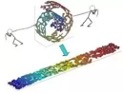
\includegraphics[width=1\linewidth]{figures-pca/dim_reduction_vis1.jpg}
\end{minipage}

\begin{figure}
\centering
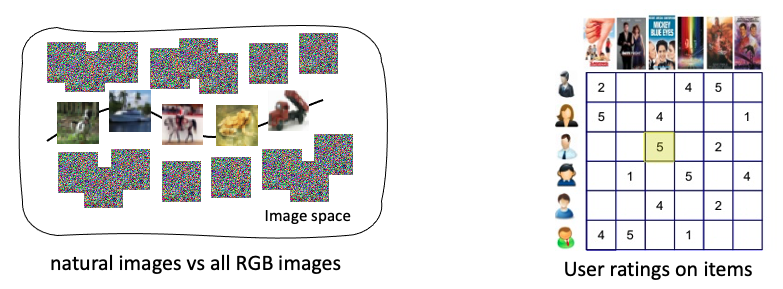
\includegraphics[width=0.9\linewidth]{figures-pca/dim_reduction_vis2.png}
\end{figure}

\end{frame}


\begin{frame}{Dimensionality reduction}
To name a few dimensionality reduction methods:

\begin{figure}
\centering
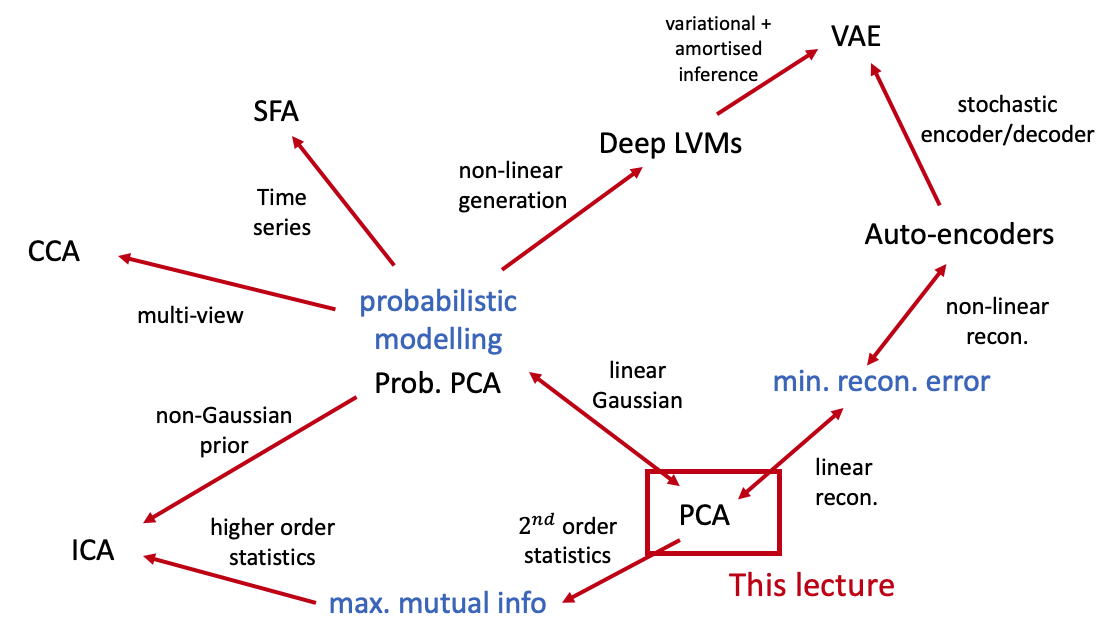
\includegraphics[width=0.9\linewidth]{figures-pca/dim_reduction_methods_vis2.png}
\end{figure}

\end{frame}

\begin{frame}{PCA in practise}

\begin{figure}
\centering
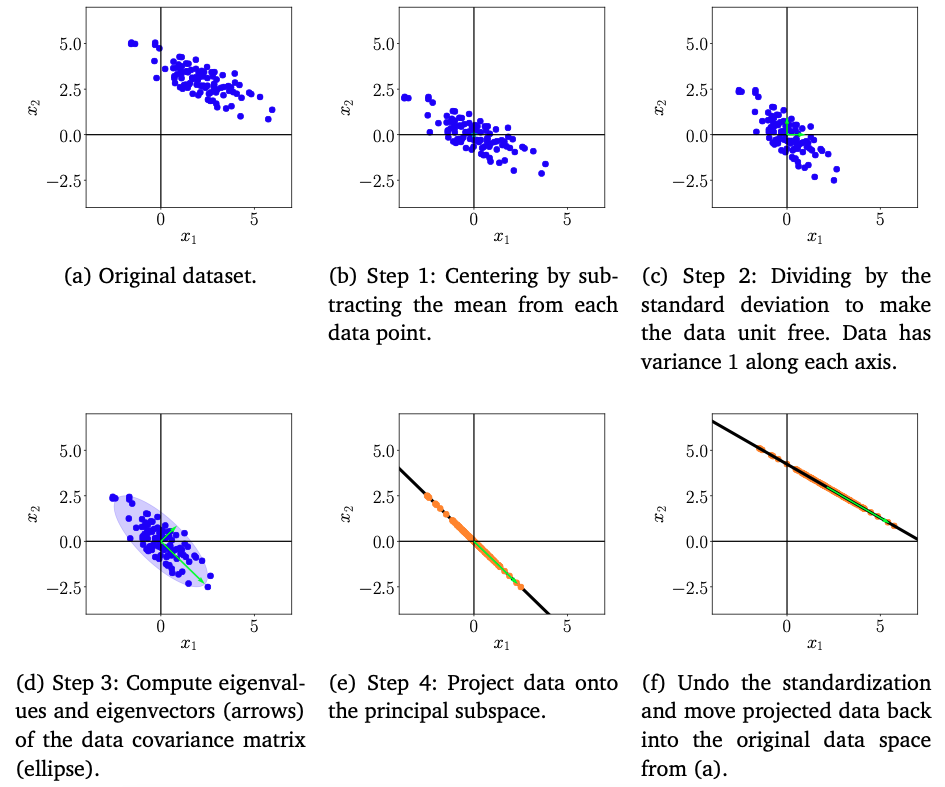
\includegraphics[width=0.7\linewidth]{figures-pca/keysteps_pca.png}
\end{figure}
\hfill \tiny{Fig from the MML book.}

\end{frame}



\begin{frame}{PCA: set-up}
Problem set-up:
\begin{itemize}
\item Data: $\data = \{\x_1, ..., \x_N \}$, $\x_n \in \mathbb{R}^{D\times 1}$ s.t. $\text{mean}(\x_n) = \bm{0}$
\item Find projections in a \alert{lower-dimensional} space: 
$$\x_n \approx \tilde{\x}_n := \sum_{j=1}^{\textcolor{red}{M}} \z_{nj} \Bb_j, \quad \z_{nj} := \Bb^\top_j \x_n$$
using an \alert{orthonormal basis}
$$\BB = [\Bb_1, ..., \Bb_M], \quad \Bb_m \in \mathbb{R}^{D \times 1}, \quad \textcolor{red}{M < D}$$
\end{itemize}

\end{frame}


\begin{frame}{Quick refresher: basis}

For a given datapoint $\x_n = [\x_{n1}, ..., \x_{nD}]^\top \in \mathbb{R}^{D\times 1}$

\begin{figure}
\centering
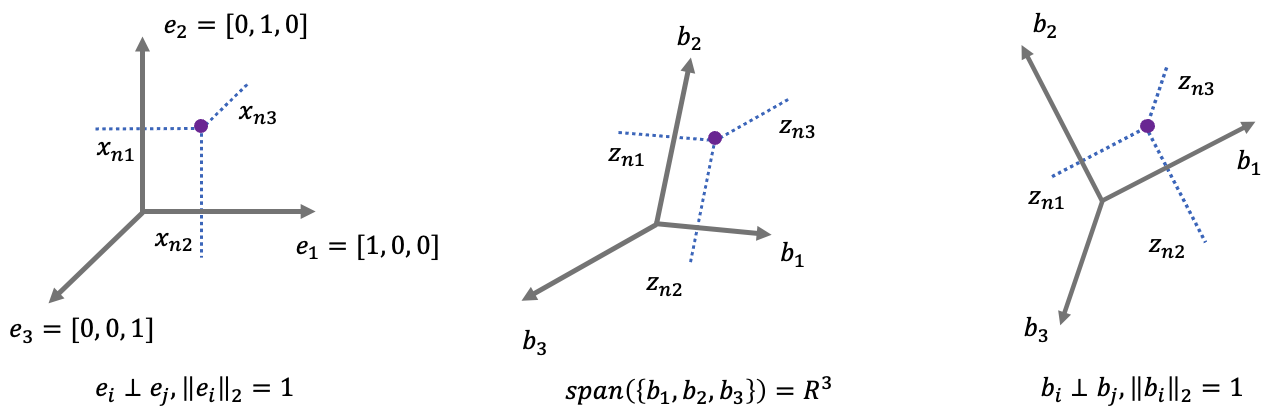
\includegraphics[width=1\linewidth]{figures-pca/basis_visual.png}
\end{figure}
\vspace{-1em}
\hfill \footnotesize{$\uparrow$ orthonormal basis}

Coordinates $\{ \z_{nj} \}$ are projections of the $\x_n$ vector onto a given basis:
$$\x_n = \sum_{j=1}^D \z_{nj} \Bb_j, \quad \z_{nj} := \Bb_j^\top \x_n$$
\end{frame}


%%%%%%%%%%%%%%%%%%%%%%
\begin{frame}{PCA: maximum variance perspective}

The ``maximum variance'' intuition of PCA:

project onto directions where the datapoints ``vary the most''

\begin{minipage}{0.5\linewidth}
\only<1>{
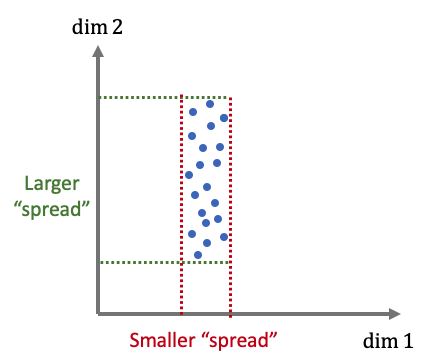
\includegraphics[width=0.8\linewidth]{figures-pca/pca_variance_intuition1.png}
}
\only<2->{
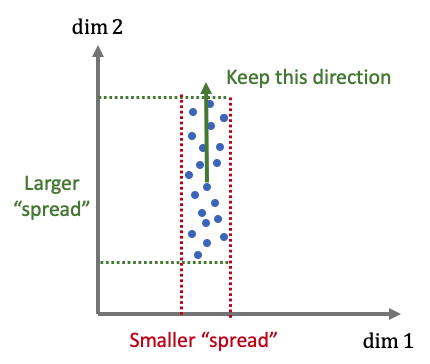
\includegraphics[width=0.8\linewidth]{figures-pca/pca_variance_intuition2.png}
}
\end{minipage}
\hfill
\begin{minipage}{0.45\linewidth}
\only<3>{
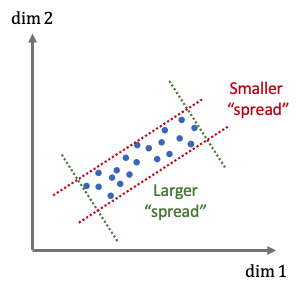
\includegraphics[width=0.8\linewidth]{figures-pca/pca_variance_intuition3.png}
}
\only<4>{
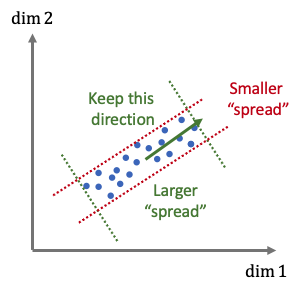
\includegraphics[width=0.8\linewidth]{figures-pca/pca_variance_intuition4.png}
}
\end{minipage}
\vspace{1em}

``Spread'' is defined as the variance along a given direction

\end{frame}

\begin{frame}{PCA: maximum variance perspective}
Problem set-up:
\begin{itemize}
\item Data: $\data = \{\x_1, ..., \x_N \}$, $\x_n \in \mathbb{R}^{D\times 1}$ s.t. $\text{mean}(\x_n) = \bm{0}$
\item Find projections in a \alert{lower-dimensional} space: 
$$\z_n := \BB^\top \x_n  \quad \Leftrightarrow \quad \z_{nj} := \Bb^\top_j \x_n $$
using an \alert{orthonormal basis}
$$\BB = [\Bb_1, ..., \Bb_M], \quad \Bb_m \in \mathbb{R}^{D \times 1}, \quad \textcolor{red}{M < D}$$
\item Solve for $\Bb_1$ such that
$$ \mathbb{V}[\Bb_1^\top \x_n] \quad \text{is maximised}$$
\end{itemize}

\end{frame}

\begin{frame}{PCA: maximum variance perspective}
Solve for $\Bb_1$ such that
$$ \mathbb{V}[\Bb_1^\top \x_n] \quad \text{is maximised,    subject to } || \Bb_1 ||_2 = 1$$

\vspace{-0.5em}
\begin{itemize}
\item Variance after projection (recall that $\x_n$ has mean zero): 
\begin{equation*}
\begin{aligned}
\mathbb{V}[\Bb_1^\top \x_n] &:= \frac{1}{N} \sum_{n=1}^N (\Bb_1^\top \x_n)^2 = \Bb_1^\top (\textcolor{red}{\underbrace{\frac{1}{N}\sum_{n=1}^N \x_n \x_n^\top}_{:=\BS = \BQ \Lambda \BQ^\top }} ) \Bb_1 \\
&= \Bb_1^\top \BQ \Lambda \underbrace{\BQ^\top \Bb_1}_{:= \bm{\beta}_1} = \sum_{d=1}^D \lambda_d \beta_{1d}^2
\end{aligned}
\end{equation*}

\item $|| \Bb_1 ||_2^2 = 1 \quad \Rightarrow \quad || \bm{\beta}_1 ||_2^2 = 1$ 
\begin{equation*}
|| \Bb_1 ||_2^2 := \Bb_1^\top \Bb_1 = \Bb_1^\top \textcolor{red}{\underbrace{\BQ \BQ^\top}_{=\mathbf{I}}} \Bb_1 = (\BQ^\top \Bb_1 )^\top (\underbrace{\BQ^\top \Bb_1}_{:= \bm{\beta}_1} ) =  \bm{\beta}_j^\top \bm{\beta}_j = || \bm{\beta}_1 ||_2^2
\end{equation*}

\end{itemize}

\end{frame}

\begin{frame}{PCA: maximum variance perspective}
Solve for $\Bb_1$ such that
$$ \mathbb{V}[\Bb_1^\top \x_n] \quad \text{is maximised,    subject to } || \Bb_1 ||_2 = 1$$

\begin{itemize}
\item Equivalent to solving the following problem 
$$ \max_{\bm{\beta}_1} \sum_{d=1}^D \lambda_d \beta_{1d}^2 \quad \text{ s.t.} || \bm{\beta}_1 ||_2^2 = \sum_{d=1}^D \beta_{1d}^2 = 1.$$


\item \alert{Solution: $\bm{\beta}_1 = \bm{e}_1 := (1, 0, ..., 0)^\top$} \\ $\Rightarrow \Bb_1 = \bm{q}_1$ (the eigenvector with the largest eigenvalue)
\end{itemize}

\end{frame}


\begin{frame}{PCA: maximum variance perspective}
Iteratively solve for the rest of the directions $\Bb_2, ... \Bb_M$:

For $m = 2, ..., M$: 
\begin{itemize}
\item Compute the ``remainder'' of projection: 
$$\textcolor{red}{\hat{\x}_n} = \x_n - \sum_{j=1}^{m-1} \z_{nj} \Bb_j = \x_n - \sum_{j=1}^{m-1} (\Bb_j^\top \x_n) \Bb_j$$ \pause

\item maximise the following objective w.r.t.~$\Bb_m$: 
$$\max_{\Bb_m} \mathbb{V}[\Bb_m^\top \textcolor{red}{\hat{\x}_n}], \quad \text{s.t. } || \Bb_m ||_2 = 1, \Bb_m \perp \Bb_j, j = 1, ..., m-1$$
\end{itemize}

\end{frame}

\begin{frame}{PCA: maximum variance perspective}
Iteratively solve for the rest of the directions $\Bb_2, ... \Bb_M$:

For $m = 2, ..., M$: 

\begin{itemize}
\item maximise $\mathbb{V}[\Bb_m^\top \hat{\x}_n]$, subject to $|| \Bb_m ||_2 = 1$, $\Bb_m \perp \Bb_j, j = 1, ..., m-1$

\item Recall that $\x_n$ has mean zero:
\begin{equation*}
\begin{aligned}
\mathbb{V}[\Bb_m^\top \hat{\x}_n] &:= \frac{1}{N} \sum_{n=1}^N (\Bb_m^\top \x_n - \sum_{j=1}^{m-1} (\Bb_j^\top \x_n) \textcolor{red}{\underbrace{\Bb_j^\top \Bb_m}_{=0}})^2 = \Bb_m^\top (\textcolor{red}{ \underbrace{\frac{1}{N} \sum_{n=1}^N \x_n \x_n^\top}_{=\BS = \BQ \Lambda \BQ^\top}} ) \Bb_m \\
&= \Bb_m^\top \BQ \Lambda \underbrace{\BQ^\top \Bb_m}_{:= \bm{\beta}_m} = \sum_{d=1}^D \lambda_d \beta_{md}^2
\end{aligned}
\end{equation*}

\item Here $\Lambda = diag(\lambda_1, ..., \lambda_d)$ and $\lambda_1 \geq ... \geq \lambda_D \geq 0$.

\end{itemize}

\end{frame}


\begin{frame}{PCA: maximum variance perspective}
Iteratively solve for the rest of the directions $\Bb_2, ... \Bb_M$:

For $m = 2, ..., M$: 
\begin{itemize}
\item maximise $\mathbb{V}[\Bb_m^\top \hat{\x}_n]$, subject to $|| \Bb_m ||_2 = 1$, $\Bb_m \perp \Bb_j, j = 1, ..., m-1$

\item $|| \Bb_m ||_2^2 = 1 \quad \Rightarrow \quad || \bm{\beta}_m ||_2^2 = 1$ 
\begin{equation*}
\hspace{-1em}
|| \Bb_m ||_2^2 := \Bb_m^\top \Bb_m = \Bb_m^\top \textcolor{red}{\underbrace{\BQ \BQ^\top}_{=\mathbf{I}}} \Bb_m = (\BQ^\top \Bb_m )^\top (\underbrace{\BQ^\top \Bb_m}_{:= \bm{\beta}_m} ) =  \bm{\beta}_m^\top \bm{\beta}_m = || \bm{\beta}_m ||_2^2
\end{equation*}

\item $\Bb_m \perp \Bb_j \quad \Rightarrow \quad \Bb_m^\top \Bb_j = 0 \quad \Rightarrow \quad \bm{\beta}_m^\top \bm{\beta}_j = 0$
\begin{equation*}
\Bb_m^\top \Bb_j = \Bb_m^\top \textcolor{red}{\underbrace{\BQ \BQ^\top}_{=\mathbf{I}}} \Bb_j = (\underbrace{\BQ^\top \Bb_m}_{:= \bm{\beta}_m} )^\top (\underbrace{\BQ^\top \Bb_j}_{:= \bm{\beta}_j} ) =  \bm{\beta}_m^\top \bm{\beta}_j 
\end{equation*}

\end{itemize}
\end{frame}



\begin{frame}{PCA: maximum variance perspective}
Iteratively solve for the rest of the directions $\Bb_2, ... \Bb_M$:

For $m = 2, ..., M$:
\begin{itemize}
\item maximise $\mathbb{V}[\Bb_m^\top \x_n]$, subject to $|| \Bb_m ||_2 = 1$, $\Bb_m \perp \Bb_j, j = 1, ..., m-1$

\item Equivalent to the following optimisation problem:
$$ \max_{\bm{\beta}_m} \sum_{d=1}^D \lambda_d \beta_{md}^2 \quad \text{ s.t.} || \bm{\beta}_m ||_2^2 =1, \bm{\beta}_m^\top \bm{\beta}_j = 0, j = 1, ..., m-1.$$
\end{itemize}

Proof by induction: we show $\bm{\beta}_m = \bm{e}_m := (0, ..., 0, \underbrace{1}_{m\text{th element}}, 0, ..., 0)$

\vspace{-0.5em}
\begin{itemize}
\item[1.] $\bm{\beta}_1 = \bm{e}_1 \quad \Rightarrow \quad \Bb_1 = \bm{q}_1$ \pause
\item[2.] For $m=2, ..., M$, assume $\bm{\beta}_j = \bm{e}_j, j = 1, ..., m-1$
\begin{itemize}
	\item[2a.] $\bm{\beta}_m^\top \bm{\beta}_j = 0, j = 1, ..., m-1 \quad \Rightarrow \quad \bm{\beta}_{mj} = 0, j = 1, ..., m-1$ \pause
	\item[2b.] $||\bm{\beta}_m ||_2 = 1 \quad \Rightarrow \quad \sum_{d=m}^D \beta_{md}^2 = 1$ \pause
	\item[2c.] Solve for maximum of $\sum_{d=m}^D \lambda_d \beta_{md}^2$ w.r.t.~$\beta_{md}$:
	\\ \alert{Solution: $\bm{\beta}_m = \bm{e}_m \quad \Rightarrow \quad \Bb_m = \bm{q}_m$}
\end{itemize}
\end{itemize}

\end{frame}


\begin{frame}{PCA: maximum variance perspective}

For $m = 1, ..., M$:
\begin{itemize}
\item maximise $\mathbb{V}[\Bb_m^\top \x_n]$, subject to $|| \Bb_m ||_2 = 1$, $\Bb_m \perp \Bb_j, j = 1, ..., m-1$
\end{itemize}

\alert{Solutions:} $\Bb_m = \bm{q}_m$ for $m = 1, ..., M$

$\Rightarrow$ Projecting $\x_n$ to a subspace 
$$span(\{ \bm{q}_m \}_{m=1}^M) = span(\{ \bm{q}_j \}_{j=M+1}^D)^{\perp}$$

\vspace{-1em}
\begin{minipage}{0.7\linewidth}
\begin{equation*}
\x_n = \textcolor{blue}{\underbrace{\sum_{j=1}^M \z_{nj} \bm{q}_j }_{:= \tilde{\x}_n}} + \textcolor{red}{\underbrace{\sum_{j=M+1}^D \z_{nj} \Bb_j}_{\text{dropped}}}, \quad \Bb_i \perp \bm{q}_j
\end{equation*}
$$\tilde{\x}_n \in span(\{ \bm{q}_m \}_{m=1}^M)$$
\end{minipage}
\hfill
\begin{minipage}{0.25\linewidth}
\centering
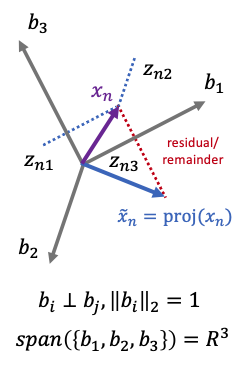
\includegraphics[width=0.9\linewidth]{figures-pca/pca_recon_intuition2.png}
\end{minipage}

\end{frame}


%%%% PCA: minimum error view

\begin{frame}{PCA: minimum reconstruction error perspective}

Goal: find orthonormal basis $\{\Bb_1, ..., \Bb_M \}$ to minimise $\ell_2$ reconstruction error:
\begin{equation*}
L = \frac{1}{N} \sum_{n=1}^N || \x_n - \tilde{\x}_n ||_2^2, \quad \tilde{\x}_n := \sum_{j=1}^M \z_{nj} \Bb_j, \ \z_{nj} = \Bb_j^\top \x_n.
\end{equation*}

Rewriting the loss:

\begin{minipage}{0.7\linewidth}

\begin{itemize}
\item Consider the full orthonormal basis:
$$\BB_{full} = [ \underbrace{\Bb_1, ..., \Bb_M}_{\text{will be used in new basis}}, \underbrace{\Bb_{M+1}, ..., \Bb_{D}}_{\text{will be dropped}}]$$
\vspace{-1em}
\item Representing $\x_n$ using basis $\BB_{full}$:
\end{itemize}
\only<1>{
\begin{equation*}
\x_n = \textcolor{blue}{\underbrace{\sum_{j=1}^M \z_{nj} \Bb_j }_{:= \tilde{\x}_n} } + \textcolor{red}{ \sum_{j=M+1}^D \z_{nj} \Bb_j}, \quad \z_{nj} := \Bb^\top_j \x_n
\end{equation*}
}
\only<2>{
\begin{equation*}
\x_n - \textcolor{blue}{\tilde{\x}_n} = \textcolor{red}{ \sum_{j=M+1}^D \z_{nj} \Bb_j}, \quad \z_{nj} := \Bb^\top_j \x_n
\end{equation*}
}

\end{minipage}
\hfill
\begin{minipage}{0.25\linewidth}

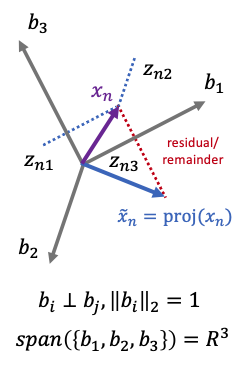
\includegraphics[width=1\linewidth]{figures-pca/pca_recon_intuition2.png}

\end{minipage}

\end{frame}

\begin{frame}{PCA: minimum reconstruction error perspective}

Goal: find orthonormal basis $\{\Bb_1, ..., \Bb_M \}$ to minimise $\ell_2$ reconstruction error:
\begin{equation*}
L = \frac{1}{N} \sum_{n=1}^N || \x_n - \tilde{\x}_n ||_2^2, \quad \tilde{\x}_n := \sum_{j=1}^M \z_{nj} \Bb_j, \ \z_{nj} = \Bb_j^\top \x_n.
\end{equation*}

Rewriting the loss:

\only<1>{
First notice that $\BB_{full}$ is an \alert{orthonormal} basis:
\begin{equation*}
\begin{aligned}
L &= \frac{1}{N} \sum_{n=1}^N || \sum_{j=M+1}^D \z_{nj} \Bb_j ||_2^2 \\
&= \frac{1}{N} \sum_{n=1}^N \sum_{j=M+1}^D || \z_{nj} \Bb_j ||_2^2 \\
&= \frac{1}{N} \sum_{n=1}^N \sum_{j=M+1}^D \z_{nj}^2
\end{aligned}
\end{equation*}
}

\only<2>{
Plugging-in that $\z_{nj} = \Bb_j^\top \x_n$:
\begin{equation*}
\begin{aligned}
L &= \frac{1}{N} \sum_{n=1}^N \sum_{j=M+1}^D (\Bb_j^\top \x_n)^2 = \frac{1}{N} \sum_{n=1}^N \sum_{j=M+1}^D \Bb_j^\top (\x_n \x_n^\top) \Bb_j \\
&= \sum_{j=M+1}^D \Bb_j^\top ( \textcolor{red}{\underbrace{\frac{1}{N} \sum_{n=1}^N \x_n \x_n^\top}_{:=\BS = \BQ \Lambda \BQ}}) \Bb_j = \sum_{j=M+1}^D \Bb_j^\top \BQ \Lambda \underbrace{\BQ^\top \Bb_j}_{:= \bm{\beta}_j} = \sum_{j=M+1}^D \sum_{d=1}^D \lambda_d \beta_{jd}^2
\end{aligned}
\end{equation*}
}

\end{frame}


\begin{frame}{PCA: minimum reconstruction error perspective}

Assume the eigenvalue decomposition as $\BS = \BQ \Lambda \BQ^\top$, \\
with $\Lambda = diag([\lambda_1, ..., \lambda_D]), \lambda_1 \geq \cdots \geq \lambda_D$
\begin{equation*}
\begin{aligned}
\Bb_j^\top \BS \Bb_j &= \Bb_j^\top \BQ \Lambda \BQ^\top \Bb_j := \bm{\beta}_j^\top \Lambda \bm{\beta}_j = \sum_{d=1}^D \lambda_d \beta_{jd}^2 \\
\bm{\beta}_j &:= \BQ^\top \Bb_j = [\beta_{j1}, ..., \beta_{jD}] = [\bm{q}_1^\top \Bb_j, ..., \bm{q}_D^\top \Bb_j]
\end{aligned}
\end{equation*}

\begin{itemize}
\item $|| \Bb_j ||_2^2 = 1 \quad \Rightarrow \quad || \bm{\beta}_j ||_2^2 = 1$ 
\begin{equation*}
|| \Bb_j ||_2^2 := \Bb_j^\top \Bb_j = \Bb_j^\top \textcolor{red}{\underbrace{\BQ \BQ^\top}_{=\mathbf{I}}} \Bb_j = (\BQ^\top \Bb_j )^\top (\underbrace{\BQ^\top \Bb_j}_{:= \bm{\beta}_j} ) =  \bm{\beta}_j^\top \bm{\beta}_j = || \bm{\beta}_j ||_2^2
\end{equation*}

\item $\Bb_i \perp \Bb_j \quad \Rightarrow \quad \Bb_i^\top \Bb_j = 0 \quad \Rightarrow \quad \bm{\beta}_i^\top \bm{\beta}_j = 0$
\begin{equation*}
\Bb_i^\top \Bb_j = \Bb_i^\top \textcolor{red}{\underbrace{\BQ \BQ^\top}_{=\mathbf{I}}} \Bb_j = (\underbrace{\BQ^\top \Bb_i}_{:= \bm{\beta}_i} )^\top (\underbrace{\BQ^\top \Bb_j}_{:= \bm{\beta}_j} ) =  \bm{\beta}_i^\top \bm{\beta}_j 
\end{equation*}

\end{itemize}

\end{frame}


\begin{frame}{PCA: minimum reconstruction error perspective}

\begin{equation*}
\text{min}_{\bm{\beta}_{M+1:D}} \ L  = \sum_{j=M+1}^D \sum_{d=1}^D \lambda_d \beta_{jd}^2, \quad \text{s.t.} \ || \bm{\beta}_j ||_2^2 = 1, \ \bm{\beta}_i^\top \bm{\beta}_j = 0.
\end{equation*}

An iterative approach for solutions: \\
Solve $\bm{\beta}_D$ first and then solve for $\bm{\beta}_j$ for $j = D - 1, ..., M+1$. 

\begin{itemize}
\item Optimisation objective for $\bm{\beta}_D$:
$$\text{min}_{\bm{\beta}_D} \sum_{d=1}^D \lambda_d \beta_{Dd}^2, \quad \text{s.t.} \ || \bm{\beta}_D ||_2^2 = \sum_{d=1}^D \beta_{Dd}^2 = 1 $$ 
\item Notice: $\lambda_1 \geq \cdots \geq \lambda_D$ 
\item \alert{Solution}: $\bm{\beta}_D = \bm{e}_D := (0, ..., 0, 1)^\top$ \\ 
$\Rightarrow \ \Bb_D = \bm{q}_D$ (the eigenvector with the smallest eigenvalue)
\end{itemize}

\end{frame}

\begin{frame}{PCA: minimum reconstruction error perspective}

\begin{equation*}
\text{min}_{\bm{\beta}_{M+1:D}} \ L  = \sum_{j=M+1}^D \sum_{d=1}^D \lambda_d \beta_{jd}^2, \quad \text{s.t.} \ || \bm{\beta}_j ||_2^2 = 1, \ \bm{\beta}_i^\top \bm{\beta}_j = 0.
\end{equation*}

Proof by induction: for $j = D, D - 1, ..., M+1$, $\bm{\beta}_j = \bm{e}_j$, i.e., $\Bb_j = \bm{q}_j$
 
\begin{itemize}
\item[1.] For $j = D$: $\bm{\beta}_D = \bm{e}_D$, i.e., $\Bb_D = \bm{q}_D$ 
\item[2.] For $j = D-1, ..., M+1$, assume for $i > j$, $\bm{\beta}_i = \bm{e}_i$, i.e., $\Bb_i = \bm{q}_i$ 

\begin{itemize}
	\item[2a.] $\bm{\beta}_i^\top \bm{\beta}_j = 0, i > j \quad \Rightarrow \quad \bm{\beta}_j = (\beta_{j1}, ..., \beta_{jj}, 0, ..., 0)^\top$ \pause
	\item[2b.] $||\bm{\beta}_j ||^2_2 = 1 \quad \Rightarrow \quad \sum_{d=1}^j \beta_{jd}^2 = 1$ \pause
	\item[2c.] Solve for the following minimisation problem w.r.t.~$\beta_{jd}$:
	\only<4>{
	$$\text{min}_{\bm{\beta}_j} \sum_{d=1}^j \lambda_d \beta_{jd}^2, \quad \text{s.t.} \ \sum_{d=1}^j \beta_{jd}^2 = 1 $$
	}
	\only<5->{
	\\ \alert{Solution: $\bm{\beta}_j = \bm{e}_j$, i.e., $\Bb_j = \bm{q}_j$ }
	}
\end{itemize}
\end{itemize}

\end{frame}

\begin{frame}{PCA: minimum reconstruction error perspective}

\vspace{-1em}
\begin{equation*}
\begin{aligned}
\text{min}_{\BB_{full}} \ L  = \frac{1}{N} \sum_{n=1}^N || \x_n - \tilde{\x}_n ||_2^2, \quad \tilde{\x}_n := \sum_{j=1}^M \z_{nj} \Bb_j \\ 
\text{s.t.} \ || \Bb_j ||_2^2 = 1, \Bb_i \perp \Bb_j
\end{aligned}
\end{equation*}

\alert{Solutions:} $\Bb_j = \bm{q}_j$ for $j = M+1, ..., D$

$\Rightarrow$ Projecting $\x_n$ to an orthogonal complement space 
$$span(\{ \bm{q}_j \}_{j=M+1}^D)^{\textcolor{red}{\perp}} = \{ \x \in \mathbb{R}^{D\times 1}: \x^\top \bm{q}_j = 0, j = M+1, ..., D \}$$

\vspace{-1em}
\begin{minipage}{0.7\linewidth}
\begin{equation*}
\x_n = \textcolor{blue}{\underbrace{\sum_{j=1}^M \z_{nj} \Bb_j }_{:= \tilde{\x}_n}} + \textcolor{red}{\underbrace{\sum_{j=M+1}^D \z_{nj} \bm{q}_j}_{\text{dropped}}}, \quad \Bb_i \perp \bm{q}_j
\end{equation*}
$$\tilde{\x}_n \in span(\{ \bm{q}_j \}_{j=M+1}^D)^{\textcolor{red}{\perp}}$$
\end{minipage}
\hfill
\begin{minipage}{0.25\linewidth}
\centering
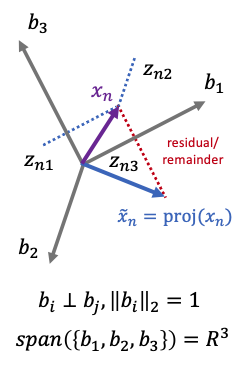
\includegraphics[width=0.9\linewidth]{figures-pca/pca_recon_intuition2.png}
\end{minipage}

\end{frame}

%%%%%%%%

\begin{frame}{PCA: comparing both views}
\begin{itemize}
%
\item Maximum variance view:
$$\BB_{full}^* = \{ \bm{q}_1, ..., \bm{q}_M, \Bb_{M+1}, ..., \Bb_D \}, \quad \Bb_i \perp \Bb_j, \Bb_i \perp \bm{q}_j$$ 

\item Minimum reconstruction error view:
$$\BB_{full}^* = \{ \Bb_1, ..., \Bb_M, \bm{q}_{M+1}, ..., \bm{q}_D \}, \quad \Bb_i \perp \Bb_j, \Bb_i \perp \bm{q}_j$$

\item No unique solution! By convention we often use $\BB_{full}^* = \BQ$

\item Relates to the equivalence between PCA and \emph{linear auto-encoder} \\ (exercise for you)
\end{itemize}

\end{frame}

%%%%%%%





\end{document}
%%% Local Variables: 
%%% mode: latex
%%% TeX-master: t
%%% End: 
